\section{Results}
\label{sec:results}
\vspace{-2mm}
\subsection{Experimental Setup}
\label{subsec:setup}
\paragraph{Datasets} 

We pre-train LUNA on a combined corpus of Temple University Hospital EEG Corpus (TUEG)~\citep{obeid2016temple} and the Siena Scalp EEG Database \citep{detti2020siena}, spanning recordings with 20, 22, and 29 channels amounting to over 21,900 hours of EEG data (see Table~\ref{tab:app_dataset_summary}). Downstream evaluations cover four diverse benchmarks: \textbf{TUAB} \citep{obeid2016temple}: Abnormal EEG detection (binary classification), \textbf{TUAR} \citep{obeid2016temple}: We follow prior work~\citep{ingolfsson2022} and treat artifact detection as a \emph{multiclass} (single-label) problem with five classes (one label per segment). Artifact detection (multi-class classification) \textbf{TUSL} \citep{obeid2016temple}: Slowing event classification (4-class classification). \textbf{SEED-V} \citep{liu2021comparing}: Emotion recognition (5-class classification), with unseen 62-channel topology. All subjects and recordings from the downstream evaluation datasets (TUAB, TUAR, TUSL, SEED-V) were strictly excluded from this pre-training set to ensure fair evaluation of generalization. For LUNA, the input EEG is segmented into patches, consisting of 40 timestamps. For most datasets, EEG recordings are sliced into non-overlapping 5-second segments to form individual training/evaluation samples. SEED-V dataset uses its default 1-second sample duration.

\paragraph{Fine-tuning and Data Splits}
For the TUAB dataset, we use the official train-test split. As TUSL and TUAR lack official subject-wise test splits, we follow recent leading work (e.g., EEGFormer~\citep{chen2024eegformer}) and adopt an 80\%/10\%/10\% randomized sample-level split for train/val/test to allow direct, like-for-like comparison. We acknowledge that subject-independent splits are the gold standard for assessing clinical generalization and recommend them for future benchmark comparisons. For SEED-V, fifteen trials are divided equally into train, validation, and test sets for each session. For the TUAR dataset, we adopt a multiclass classification approach, restricting to 5 distinct artifact types in a single-label setting, similar to EEGFormer~\citep{chen2024eegformer}. We optimize binary cross-entropy loss for TUAB and cross-entropy loss for other datasets. We report the mean and standard deviation of results obtained across three different random seeds.

\paragraph{Preprocessing}
We apply a minimal, standardized preprocessing pipeline to all EEG data. Signals are first bandpass filtered between 0.1 Hz and 75 Hz. A notch filter (50Hz or 60Hz) is applied to remove power-line interference. All signals are then resampled to 256 Hz. 
For TUEG, TUAB, TUAR, and TUSL datasets we construct a bipolar (“double-banana”) montage by differencing predefined longitudinal electrode pairs provided in the dataset documentation; the full list of channel pairs used is given in Appendix~\ref{app:bipolar_pairs}. Siena and SEED-V are processed in unipolar format. Finally, each channel within each sample is normalized using z-score normalization.

\paragraph{Computational Environment}
All experiments were conducted on a cluster of eight NVIDIA A100 GPUs, using Python 3.11.6 and PyTorch 2.4.1 with CUDA 12.1. Training utilizes `bf16` mixed-precision. Detailed hyperparameters for pre-training and fine-tuning are provided in Appendix~\ref{app:exp_settings}.

\paragraph{Baselines and Variants} 
We compare against state-of-the-art supervised and self-supervised methods, including transformer-based architectures such as LaBraM~\citep{jiang2024large}, CBraMod~\citep{wang2024cbramod}, EEGFormer~\citep{chen2024eegformer}, and BIOT~\citep{yang2023biot}. LUNA is evaluated in three configurations: Base (7M), Large (43M), and Huge (311M parameters). Model size is increased by expanding the depth of the Patch-wise Temporal Encoder, the hidden embedding dimension \(E\), and the number/size of queries \(Q\) in the Channel-Unification Module. Key architectural settings are detailed in Appendix~\ref{app:model_details}.

\subsection{Downstream Task Performance}
\label{subsec:downstream_results}

\paragraph{Abnormal EEG Detection (TUAB)}
LUNA delivers competitive performance on TUAB (Table \ref{tab:results_tuab}). LUNA-Huge achieves AUROC of 0.8957 and AUPR of 0.9029, surpassing most self-supervised baselines and approaching large-scale models like LaBraM and CBraMod. Notably, LUNA maintains strong performance while offering substantial efficiency and topology-agnostic benefits relative to strong self-supervised and large-scale baselines.

\begin{table}[htbp!]
    \centering
    \caption{Performance comparison on TUAB abnormal EEG detection.}
    \label{tab:results_tuab}
    
    \setlength{\tabcolsep}{6pt} % Adjust column spacing
    \small
    \begin{tabular}{@{}lcccc@{}}
        \toprule
        \textbf{Model} & \textbf{Size} & \textbf{Bal. Acc. (\%)} $\uparrow$ & \textbf{AUC-PR} $\uparrow$ & \textbf{AUROC} $\uparrow$ \\
        \midrule
        \multicolumn{5}{l}{\textit{Supervised Models}} \\    SPaRCNet~\cite{jing2023development} & 0.8M & 78.96 $\pm$ 0.18 & 0.8414 $\pm$ 0.0018 & 0.8676 $\pm$ 0.0012 \\
        ContraWR~\cite{yang2021self} & 1.6M & 77.46 $\pm$ 0.41 & 0.8421 $\pm$ 0.0140 & 0.8456 $\pm$ 0.0074 \\
        CNN-Transformer~\cite{peh2022transformer} & 3.2M & 77.77 $\pm$ 0.22 & 0.8433 $\pm$ 0.0039 & 0.8461 $\pm$ 0.0013 \\
        FFCL~\cite{li2022motor} & 2.4M & 78.48 $\pm$ 0.38 & 0.8448 $\pm$ 0.0065 & 0.8569 $\pm$ 0.0051 \\
        ST-Transformer~\cite{song2021transformer} & 3.2M & 79.66 $\pm$ 0.23 & 0.8521 $\pm$ 0.0026 & 0.8707 $\pm$ 0.0019 \\
        \midrule
        \multicolumn{5}{l}{\textit{Self-supervised Models}} \\
        BENDR \citep{kostas2021bendr} & 0.39M & 76.96 $\pm$ 3.98 & -  & 0.8397 $\pm$ 0.0344 \\
        BrainBERT \citep{wang2023brainbert} & 43.2M & - & 0.8460 $\pm$ 0.0030 & 0.8530 $\pm$ 0.0020 \\
        EEGFormer-Base \citep{chen2024eegformer} & 2.3M & - & 0.8670 $\pm$ 0.0020 & 0.8670 $\pm$ 0.0030 \\
        BIOT \citep{yang2023biot} & 3.2M & 79.59 $\pm$ 0.57 & 0.8692 $\pm$ 0.0023 & 0.8815 $\pm$ 0.0043 \\
    EEG2Rep~\cite{mohammadi2024eeg2rep} & - & 80.52 $\pm$ 2.22 & - & 0.8843 $\pm$ 0.0309 \\
        FEMBA-Huge~\cite{tegon2025femba} & 386M  & 81.82 $\pm$ 0.16 & 0.9005 $\pm$ 0.0017 & 0.8921 $\pm$ 0.0042  \\
        CEReBrO~\cite{dimofte2025cerebro} & 85.15M & 81.67 $\pm$ 0.23 & 0.9049 $\pm$ 0.0026 & 0.8916 $\pm$ 0.0038 \\
        LaBraM-Base \citep{jiang2024large} & 5.9M & 81.40 $\pm$ 0.19 & 0.8965 $\pm$ 0.0016 & 0.9022 $\pm$ 0.0009 \\
        LaBraM-Huge \citep{jiang2024large} & 369.8M & \textbf{82.58 $\pm$ 0.11} & 0.9204 $\pm$ 0.0011 & \textbf{0.9162 $\pm$ 0.0016} \\
        CBraMod \citep{wang2024cbramod} & 69.3M & 82.49 $\pm$ 0.25 & \textbf{0.9221 $\pm$ 0.0015} & 0.9156 $\pm$ 0.0017 \\
        \midrule
        \textbf{LUNA-Base} & 7M & 80.63 $\pm$ 0.08 & 0.8953 $\pm$ 0.0016 & 0.8868 $\pm$ 0.0015 \\
        \textbf{LUNA-Large} & 43M & 80.96 $\pm$ 0.10 & 0.8986 $\pm$ 0.0005 & 0.8924 $\pm$ 0.0010 \\
        \textbf{LUNA-Huge} & 311.4M & 81.57 $\pm$ 0.11 & 0.9029 $\pm$ 0.0014 & 0.8957 $\pm$ 0.0011 \\
        \bottomrule
   \end{tabular}
\end{table}
\paragraph{Artifact and Slowing Detection (TUAR and TUSL)}
LUNA delivers state-of-the-art results on TUAR and TUSL (Table \ref{tab:results_tuar_tusl}). LUNA-Huge achieves AUROC 0.921 on TUAR, outperforming FEMBA-Large and other methods. On TUSL, LUNA-Huge reaches AUROC 0.802, the highest among all compared models. 

\begin{table}[htbp!]
\centering
\caption{Performance comparison on TUAR (artifact detection) and TUSL (slowing event classification). }
\label{tab:results_tuar_tusl}

\setlength{\tabcolsep}{5pt}
\small
\begin{tabular}{@{}lccccccc@{}}
\toprule
\multirow{2}{*}{\textbf{Model}} & \multirow{2}{*}{\textbf{Size}} & \multicolumn{2}{c}{\textbf{TUAR}} & \multicolumn{2}{c}{\textbf{TUSL}} \\
\cmidrule(lr){3-4} \cmidrule(lr){5-6}
 &  & \textbf{AUROC} $\uparrow$ & \textbf{AUC-PR} $\uparrow$ & \textbf{AUROC} $\uparrow$ & \textbf{AUC-PR} $\uparrow$ \\
\midrule
\multicolumn{6}{l}{\textit{Supervised Models}} \\
EEGNet~\cite{lawhern2018eegnet}       & -  & 0.752 $\pm$ 0.006 & 0.433 $\pm$ 0.025 & 0.635 $\pm$ 0.015 & 0.351 $\pm$ 0.006  \\
EEG-GNN~\cite{tang2021self}      & - & 0.837 $\pm$ 0.022 & 0.488 $\pm$ 0.015 & 0.721 $\pm$ 0.009 & 0.381 $\pm$ 0.004  \\
GraphS4mer~\cite{tang2023modeling}  & -  & 0.833 $\pm$ 0.006 & 0.461 $\pm$ 0.024 & 0.632 $\pm$ 0.017 & 0.359 $\pm$ 0.001  \\
\midrule
\multicolumn{6}{l}{\textit{Self-supervised Models}} \\
BrainBERT \citep{wang2023brainbert}    & 43.2M  & 0.753 $\pm$ 0.012 & 0.350 $\pm$ 0.014 & 0.588 $\pm$ 0.013 & 0.352 $\pm$ 0.003  \\
EEGFormer-Base \citep{chen2024eegformer}  & 2.3M & 0.847 $\pm$ 0.014 & 0.483 $\pm$ 0.026 & 0.713 $\pm$ 0.010 & \textbf{0.393 $\pm$ 0.003}  \\
EEGFormer-Large \citep{chen2024eegformer}  & 3.2M & 0.852 $\pm$ 0.004 & 0.483 $\pm$ 0.014 & 0.679 $\pm$ 0.013 & 0.389 $\pm$ 0.003  \\
FEMBA-Base \citep{tegon2025femba}  & 47.7M & 0.900 $\pm$ 0.010 & \textbf{0.559 $\pm$ 0.002} & 0.731 $\pm$ 0.012 & 0.289 $\pm$ 0.009 \\
FEMBA-Large \citep{tegon2025femba} & 77.8M  & 0.915 $\pm$ 0.003 & 0.521 $\pm$ 0.001 & 0.714 $\pm$ 0.007 & 0.282 $\pm$ 0.010 \\
\midrule
\textbf{LUNA-Base} & 7M & 0.902 $\pm$ 0.011 	 & 0.495 $\pm$	0.010 & 0.767 $\pm$	0.023 & 0.301 $\pm$	0.003 \\
\textbf{LUNA-Large} & 43M & 0.918 $\pm$	0.003	& 0.505 $\pm$	0.010 & 0.771	$\pm$ 0.006	& 0.293	$\pm $0.021  \\
\textbf{LUNA-Huge} & 311.4M & \textbf{0.921 $\pm$	0.011}	 & 0.528 $\pm$	0.012 & \textbf{0.802 $\pm$	0.005}	& 0.289	$\pm $0.008  \\
\bottomrule
\end{tabular}

\end{table}

\paragraph{Emotion Recognition on Unseen Montage (SEED-V)}
The SEED-V benchmark tests generalization to a novel 62-channel montage, distinct from pre-training data. Results in Table \ref{tab:emotion_classification} show that while LUNA effectively operates on this unseen topology, its performance (e.g., Bal. Acc.) lags behind leading methods like CBraMod by 2-3 pp. This suggests a trade-off inherent in LUNA's design: while its query-based unification enables efficient, topology-agnostic processing across common montage variations (as demonstrated on TUAB/TUAR/TUSL), generalizing zero-shot to vastly different, high-density layouts remains challenging, possibly due to positional encoding constraints. Despite this gap, LUNA shows positive scaling from Base to Large models, underscoring its potential.

\vspace{-3mm}
\begin{table}[htbp!]
    \centering
    \caption{Performance comparison on SEED-V emotion recognition (5-classes).}
    \label{tab:emotion_classification}
    \small
    \begin{tabular}{@{}lcccc@{}}
        \toprule
        \textbf{Model} & \textbf{Size} & \textbf{Bal. Acc. (\%)} $\uparrow$ & \textbf{Cohen’s Kappa } $\uparrow$ & \textbf{Weighted F1} $\uparrow$ \\
        \midrule
         \multicolumn{5}{l}{\textit{Supervised Models}} \\
        SPaRCNet~\cite{jing2023development} &0.79M&0.2949 $\pm$ 0.0078 &0.1121 $\pm$ 0.0139 &0.2979 $\pm$ 0.0083 \\
        ContraWR~\cite{yang2021self}&1.6M&0.3546 $\pm$ 0.0105 &0.1905 $\pm$ 0.0188 &0.3544 $\pm$ 0.0121 \\
        CNN-Transformer~\cite{peh2022transformer}&3.2M&0.3678 $\pm$ 0.0078& 0.2072 $\pm$ 0.0183&0.3642 $\pm$ 0.0088 \\
        FFCL~\cite{li2022motor}  &    2.4M &0.3641 $\pm$ 0.0092 &0.2078 $\pm$ 0.0201&0.3645 $\pm$ 0.0132\\
        ST-Transformer~\cite{song2021transformer} &3.5M &0.3052 $\pm$ 0.0072 &0.1083 $\pm$ 0.0121 &0.2833 $\pm$ 0.0105 \\
						\midrule
        \multicolumn{5}{l}{\textit{Self-supervised Models}} \\
        BIOT \citep{yang2023biot} & 3.2M & 0.3837 $\pm$ 0.0187 & 0.2261 $\pm$ 0.0262 &  0.3856 $\pm$ 0.0203 \\
        LaBraM-Base \citep{jiang2024large} & 5.8M & 0.3976 $\pm$ 0.0138 & 0.2386 $\pm$ 0.0209 & 0.3974 $\pm$ 0.0111 \\
        CBraMod \citep{wang2024cbramod} & 14M & \textbf{0.4091 $\pm$ 0.0097} & \textbf{0.2569 $\pm$ 0.0151} & \textbf{0.4101 $\pm$ 0.0108} \\
        \midrule
        
        \textbf{LUNA-Base} & 7M & 0.3730 $\pm$ 0.0098 & 0.1831 $\pm$ 0.0103 & 0.3389 $\pm$ 0.0091 \\
        \textbf{LUNA-Large} & 43M & 0.3918 $\pm$ 0.0066 & 0.2073 $\pm$ 0.0045 & 0.3586 $\pm$ 0.0013 \\
        \textbf{LUNA-Huge} & 311.4M & 0.3900 $\pm$ 0.0096 & 0.2037 $\pm$ 0.0103 & 0.3506 $\pm$ 0.0047 \\
        \bottomrule
    \end{tabular}
\end{table}
Unless noted, we report mean~$\pm$~s.d.\ over matched seeds and focus on effect sizes and confidence intervals. Formal significance tests are summarized in Appendix~\ref{app:sig_tests}

\subsection{Computational Efficiency}
\label{subsec:efficiency}


\textbf{LUNA achieves substantially better calling efficiency} compared to full and alternating attention models. As shown in Figure~\ref{fig:patch_scaling}, LUNA's patch-wise attention enables thousands of temporal patches without the quadratic cost faced by LaBraM. Likewise, Figure~\ref{fig:channel_scaling} shows that LUNA maintains near-constant compute cost when channel count increases, outperforming CBraMod's $\bigO(C^2)$ scaling for dense EEG recordings. These results confirm that LUNA decouples inference cost from input montage, making it well-suited for long recordings or high-density EEG scenarios. We also consider BIOT (linear attention) as an efficiency-oriented baseline; detailed FLOPs/memory scaling versus LUNA is provided in Appendix~\ref{app:biot_scaling}. Although many public datasets use $\sim$20–30 channels, research/clinical systems often employ 64–256 channels and longer windows; LUNA’s $O(C)$ unification and reduced temporal sequence length enable such regimes where quadratic spatial attention becomes impractical.


\begin{figure}[htbp!]
    \centering
    \begin{subfigure}{\linewidth} 
        \centering
        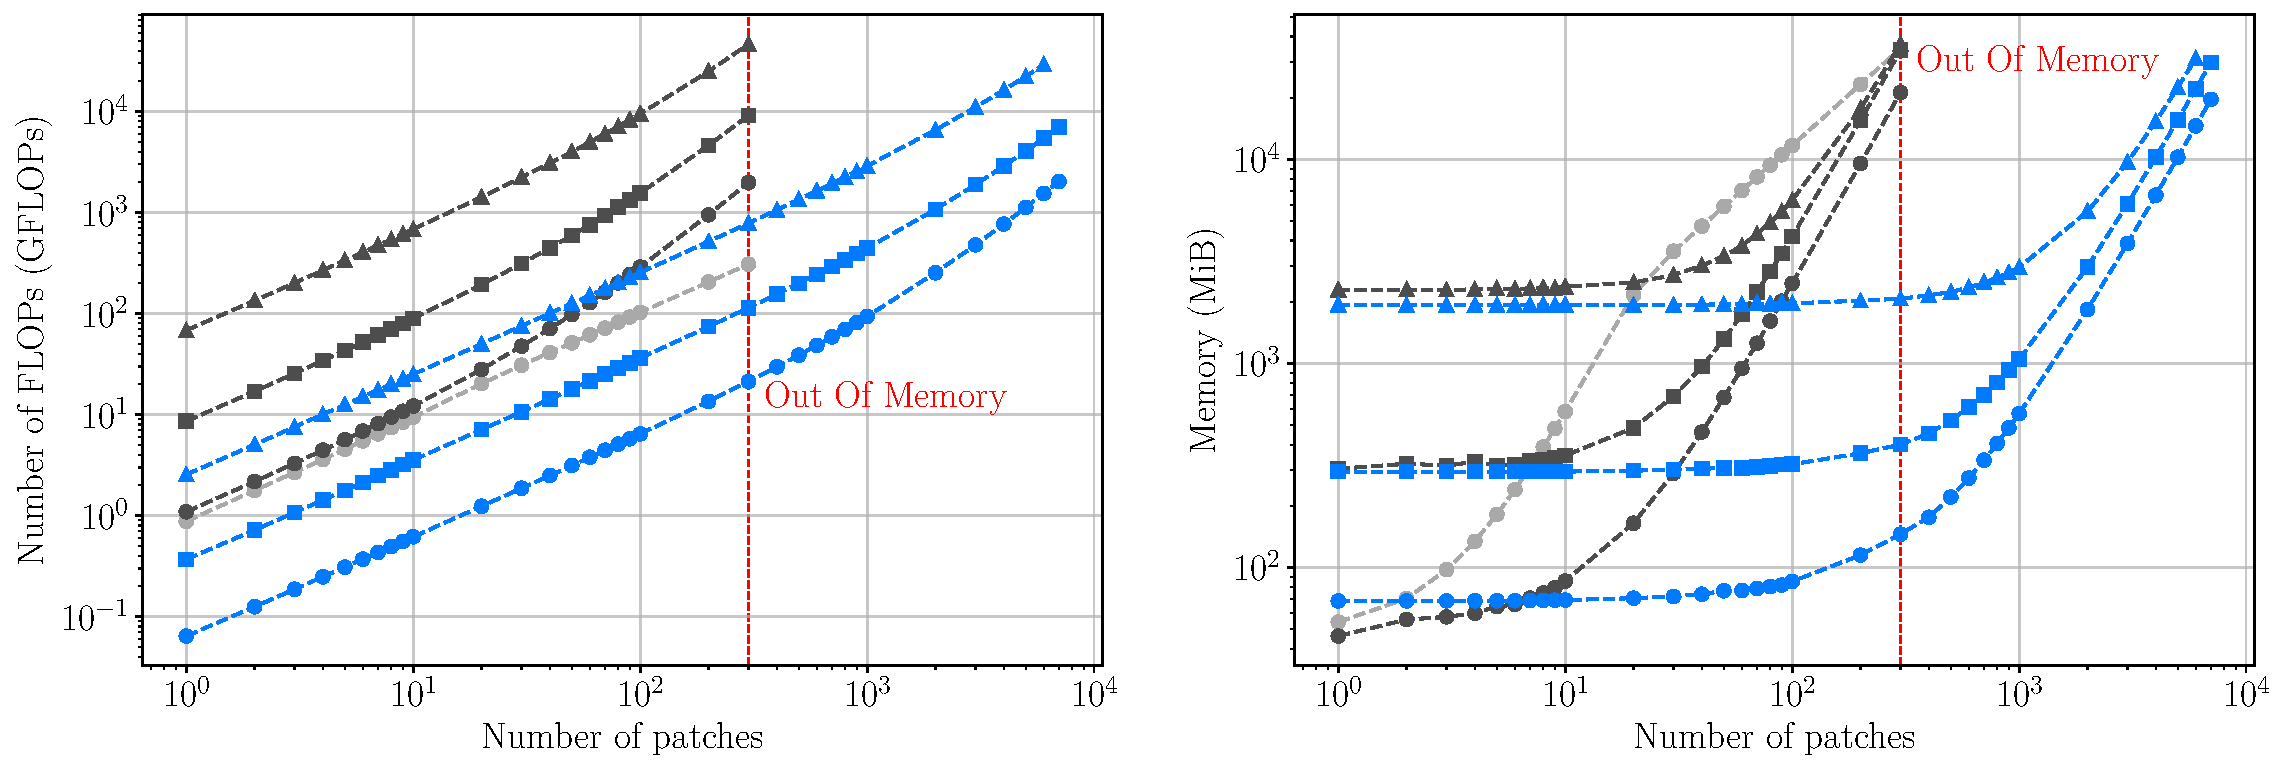
\includegraphics[width=\linewidth]{figs/scaling_plot_patches.pdf}
        \caption{Scaling with number of patches (Channels fixed at 22).}
        \label{fig:patch_scaling}
    \end{subfigure}
    \vspace{-0.2cm}

    \begin{subfigure}{\linewidth}
        \centering
        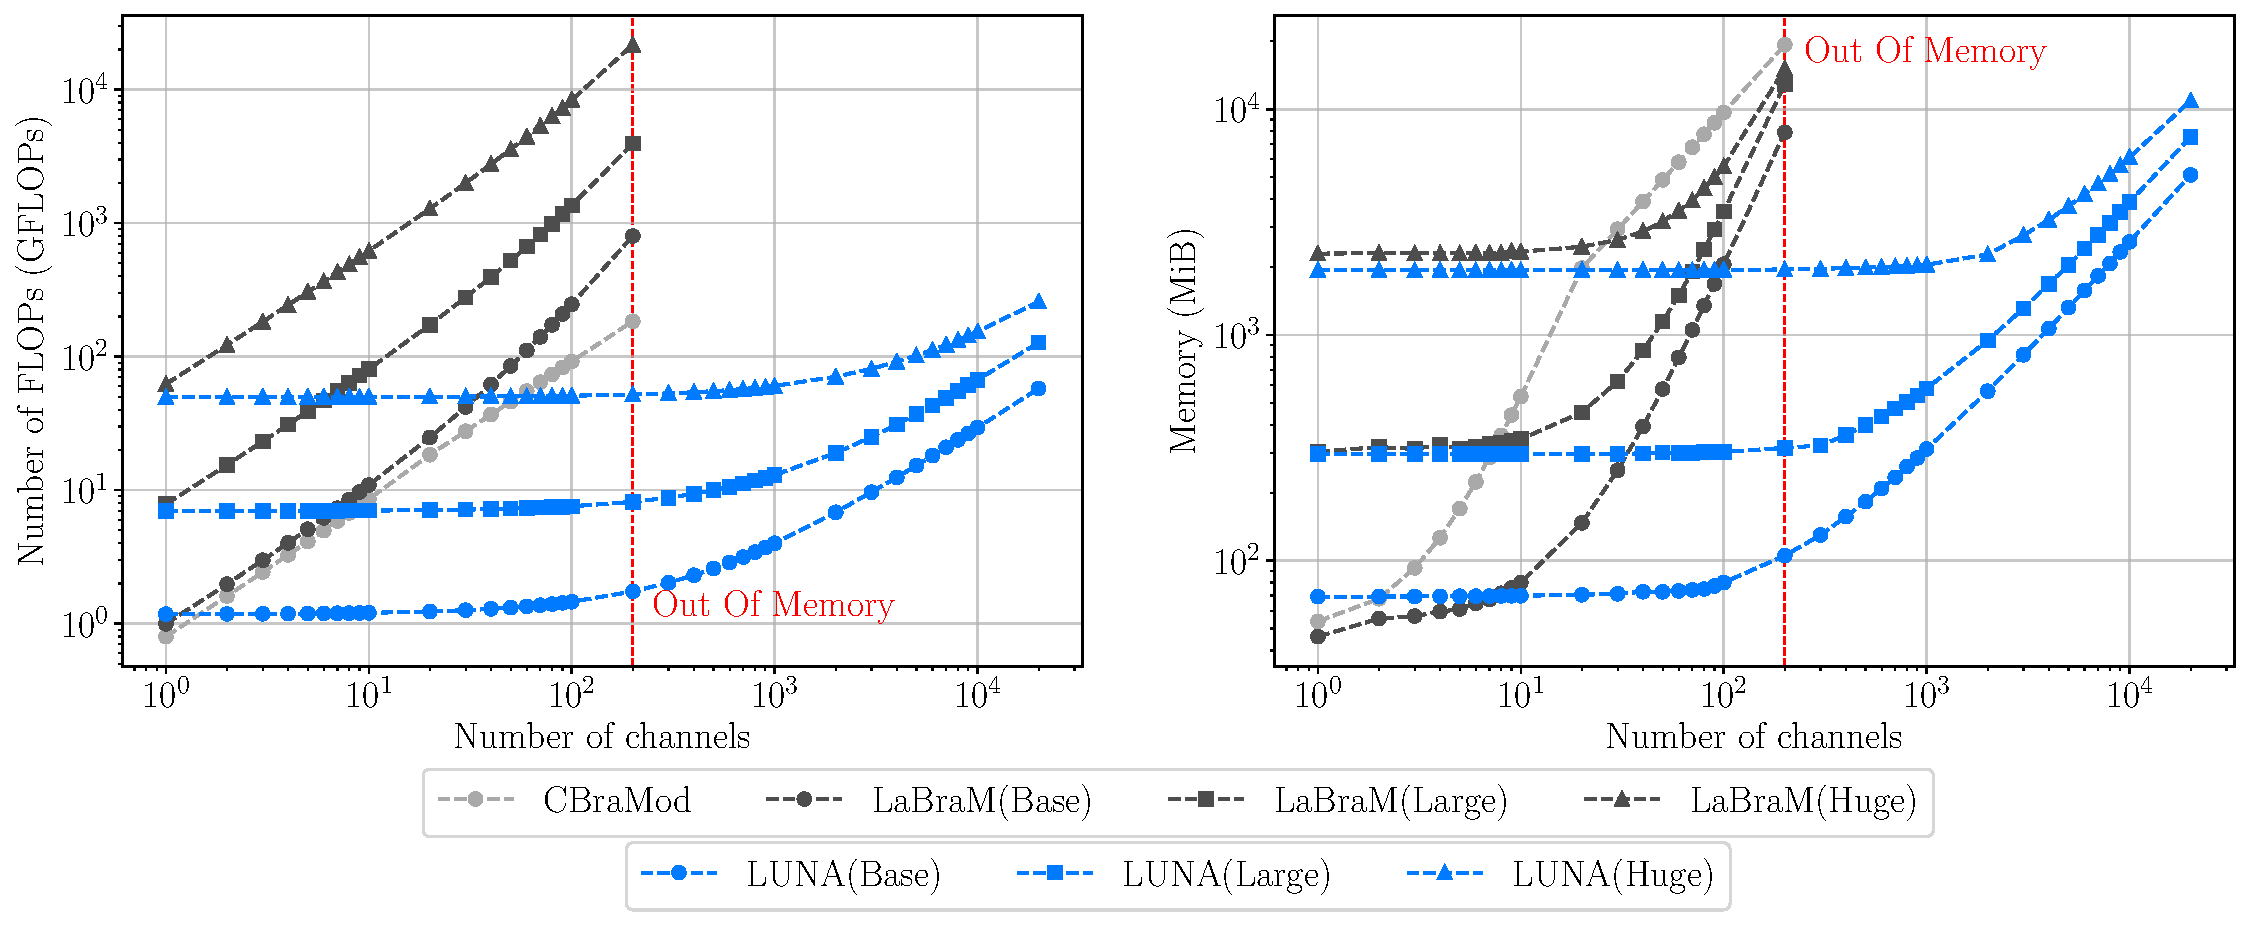
\includegraphics[width=\linewidth]{figs/scaling_plot_channels.pdf}
        \caption{Scaling with number of channels (Patches fixed at 20).}
    \label{fig:channel_scaling}
    \end{subfigure}
    \vspace{-0.6cm}
    \caption{Computational cost scaling of LUNA and baseline models. (a) FLOPs and Memory usage vs. number of patches. (b) FLOPs and Memory usage vs. number of channels. LUNA demonstrates significantly better efficiency and scalability, especially compared to full attention (LaBraM), and favorable scaling compared to alternating attention (CBraMod) due to the fixed latent query space. CBraMod has a variable sized decoder based on the number of patches and channels; therefore, its model size as well as its resource usage grows rapidly. \emph{FLOPs are measured with \texttt{fvcore}'s \texttt{FlopCountAnalysis} over 50 random inputs, including encoder{+}decoder, with window length $T$, patch size $P$, and reported as GFLOPs per forward pass.}}
    \vspace{-0.7cm}
\label{fig:scaling_plots_combined}
\end{figure}

\subsection{Ablation Studies}
\label{subsec:ablations}
\emph{Choice of $Q$.} We explore the trade-off between the number of queries $Q$ and embedding size $E$ under a fixed $Q\!\cdot\!E$ budget; see Appendix~\ref{app:q_tradeoff}. We validate the impact of LUNA's key design choices on TUAB and TUAR (Table \ref{tab:ablation}).

\vspace{-4mm}
\paragraph{Learned Queries vs. Fixed Regions}
Replacing learned queries with predefined spatial regions (similar to MMM~\citep{yi2023learning}) yields small AUROC changes ($-0.004$ to $-0.006$), within seed variation. We therefore emphasize the \emph{practical} advantages of learned queries—data-driven flexibility without anatomy-specific priors—rather than a statistically significant metric gain (Appendix~\ref{app:sig_tests}).

\vspace{-4mm}
\paragraph{Query Specialization Loss}
Removing the specialization loss results in modest AUROC changes (-0.003 to -0.006), again on the order of the reported variation, with small mixed effects on AUC-PR. We retain this loss for its \emph{regularizing role}: it encourages a diverse, non-redundant set of spatial filters (see Fig.~\ref{fig:query_analysis}), which is desirable for robustness in challenging artifact conditions.

\vspace{-4mm}
\paragraph{Frequency Features}
Ablating frequency embeddings leads to the largest drop (up to -0.012 AUROC), indicating a more consistent contribution complementary to temporal features.


\subsection{Latent Space Analysis}
\paragraph{Pre-trained Representations}
t-SNE visualizations (Figure~\ref{fig:app_tsne_plots}) reveal that even before fine-tuning, LUNA's encoder captures task-relevant structure. Normal and abnormal EEGs form separate clusters in TUAB, while artifact classes are partially separated in TUAR, demonstrating effective pre-training.


\begin{figure}[htbp!]
    \centering
    \begin{subfigure}[b]{0.48\textwidth}
        \centering
        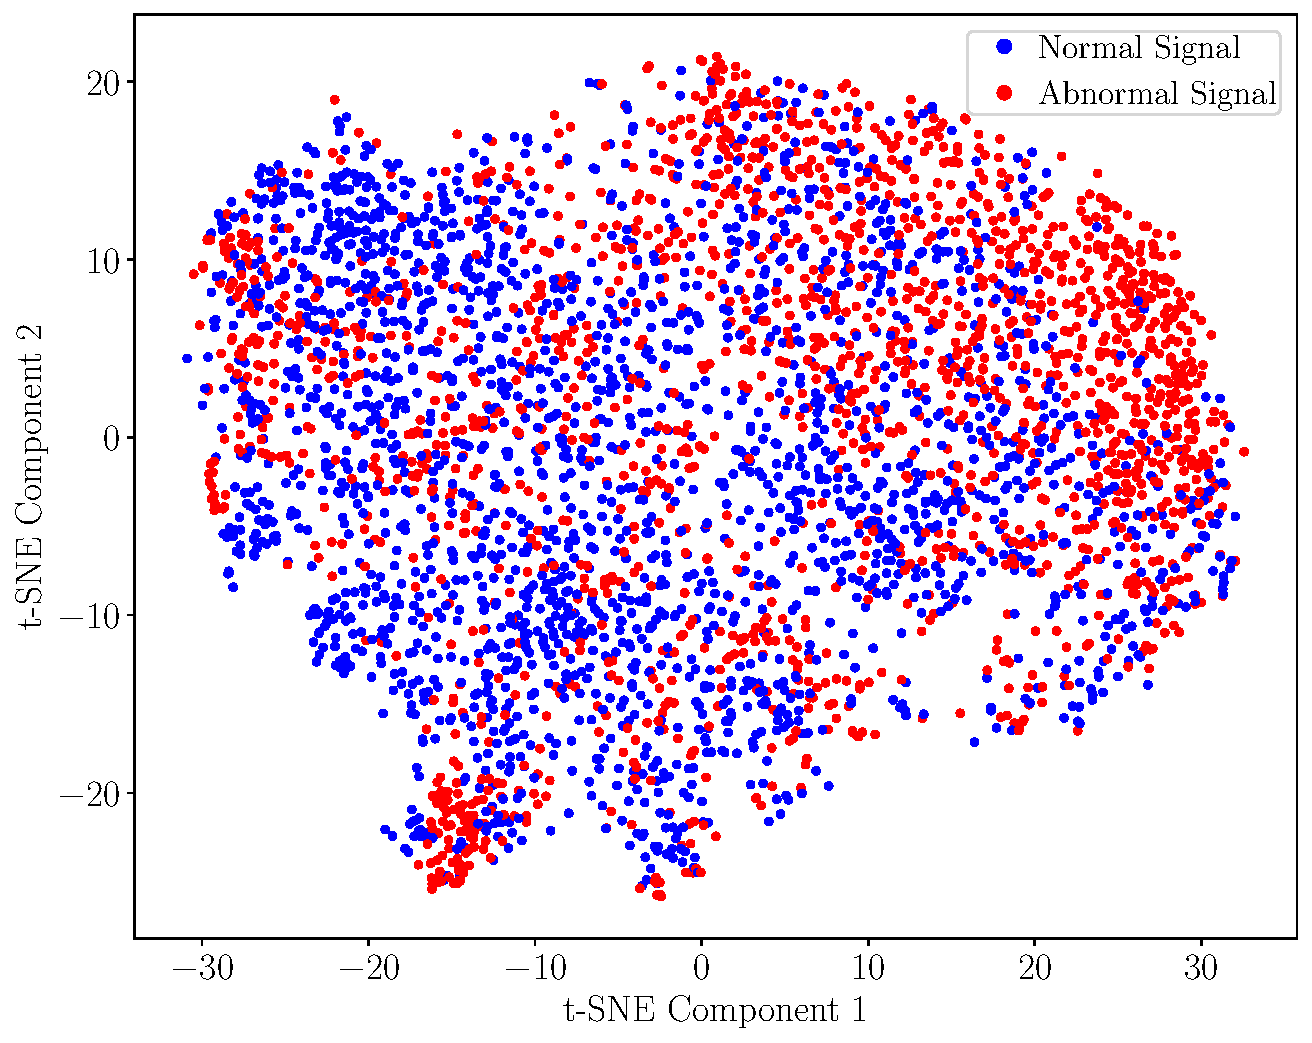
\includegraphics[width=\linewidth]{figs/t-SNE_tuab.pdf}
        \caption{TUAB dataset (Normal vs. Abnormal Signal).}
        \label{fig:app_TUAB_emb}
    \end{subfigure}
    \hfill 
    \begin{subfigure}[b]{0.48\textwidth}
        \centering
        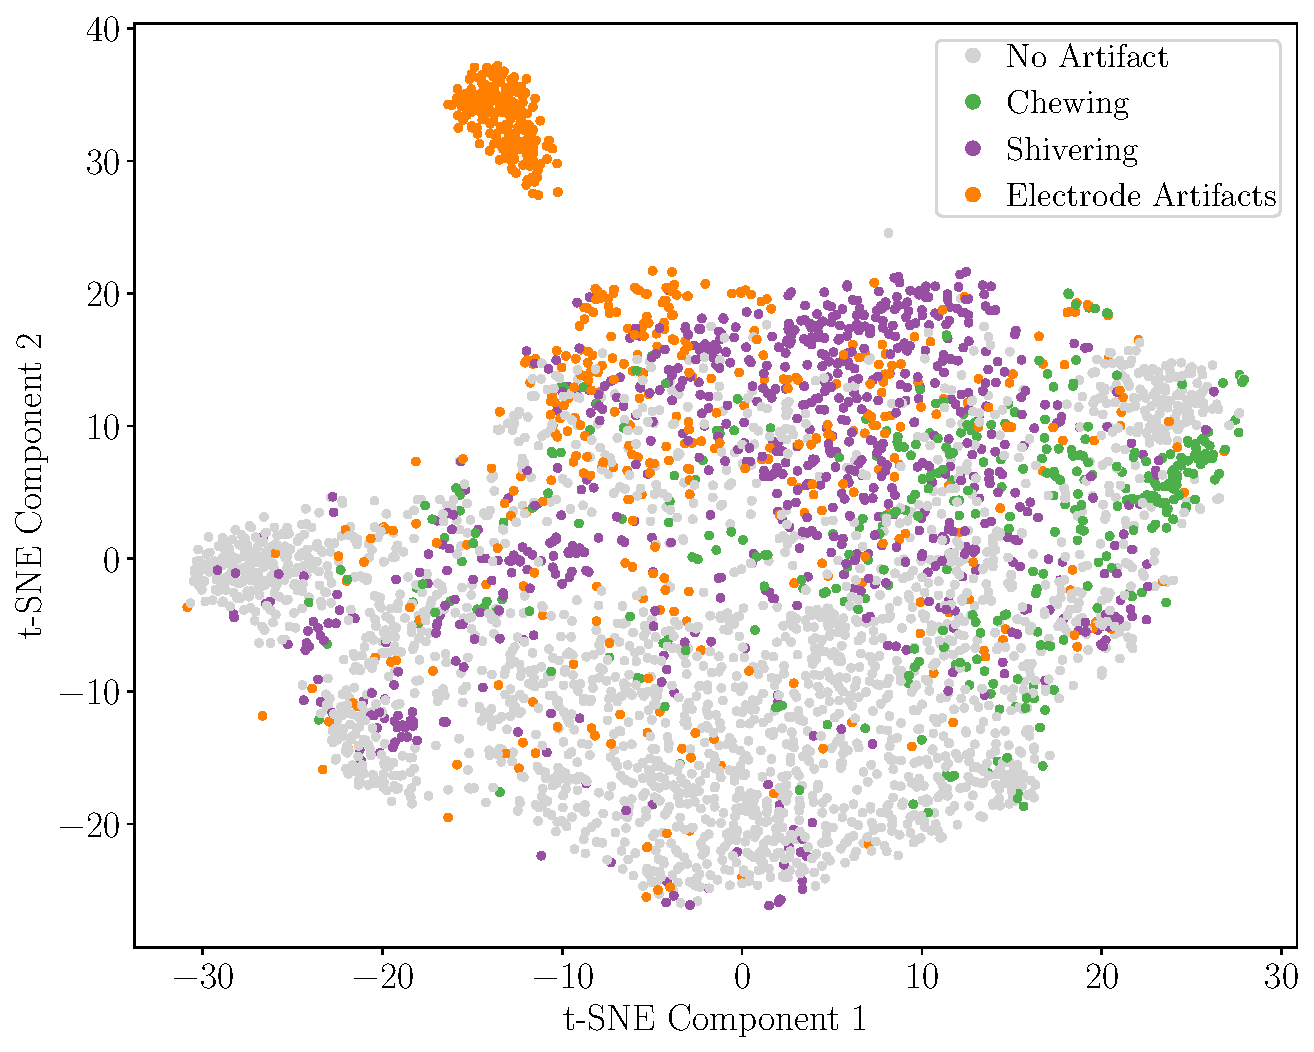
\includegraphics[width=\linewidth]{figs/t-SNE_tuar.pdf} 
        \caption{TUAR dataset (Artifact Types).}
        \label{fig:app_TUAR_emb}
    \end{subfigure}
    \caption{t-SNE of LUNA-Base embeddings on downstream datasets before fine-tuning.}
    \label{fig:app_tsne_plots} 
    \vspace{-0.5cm}
\end{figure}

\subsection{Learned Query Specialization Visualization}
\label{subsec:qualitative}

\paragraph{Query Specialization}
Visual analysis of the learned queries (Figure~\ref{fig:query_analysis}) highlights their role in topology-agnostic representation. Queries exhibit distinct spatial profiles: some are localized (e.g., frontal regions), while others aggregate broader signals. This emergent specialization confirms that cross-attention learns flexible, data-driven basis functions for spatial unification.

\begin{figure}[htbp!]
    \vspace{-0.2cm}
    \centering
    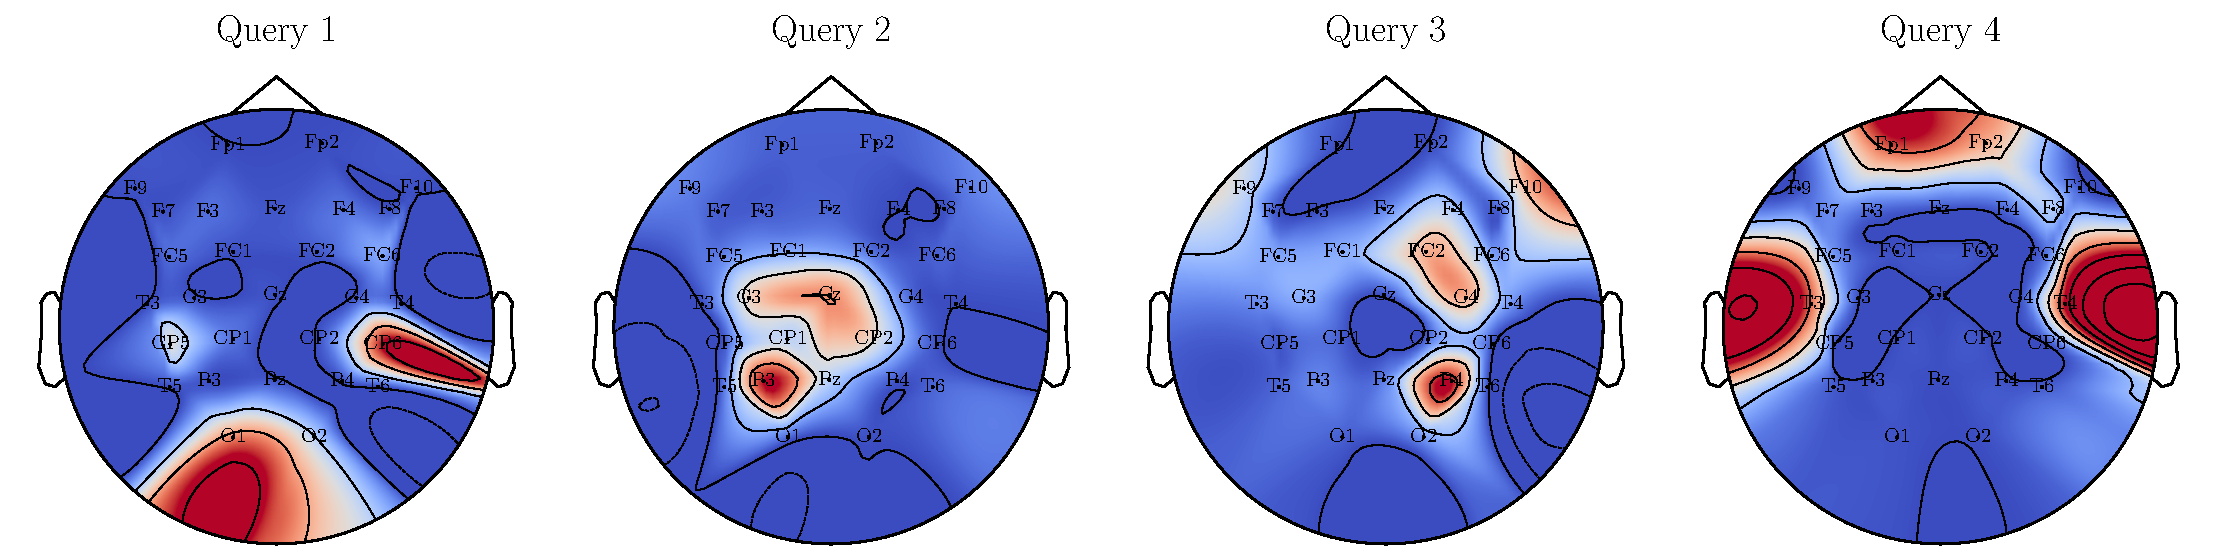
\includegraphics[width=1\linewidth]{figs/query_analysis_small.pdf}
    \caption{Visualization of the attention patterns of queries in LUNA-Base on Siena~\citep{detti2020siena} topology.}
    \label{fig:query_analysis}
    \vspace{-0.2cm}
\end{figure}

\begin{table}[htbp!]
    \centering
    \vspace{-0.4cm}
   \caption{Ablation study results (LUNA-Base) on TUAB and TUAR datasets.}
    \label{tab:ablation}
    \scriptsize
    \setlength{\tabcolsep}{2pt}
    \begin{tabular}{@{}lcccc@{}}
        \toprule
        \textbf{Model Configuration} & \textbf{TUAB AUROC} & \textbf{TUAB AUC-PR} & \textbf{TUAR AUROC} & \textbf{TUAR AUC-PR} \\
        \midrule  
        LUNA-Base (Full Model) & 0.887 $\pm$ 0.002 & 0.895 $\pm$ 0.002 & 0.902 $\pm$ 0.011 & 0.495 $\pm$ 0.010 \\
        \midrule
        \textit{Unification Module:} \\
        \quad - Region-based Attention  & 0.883 $\pm$ 0.001 \textcolor{red}{($\downarrow$ 0.004)} & 0.892 $\pm$ 0.002 \textcolor{red}{($\downarrow$ 0.003)} & 0.896 $\pm$ 0.001 \textcolor{red}{($\downarrow$ 0.006)} & 0.509 $\pm$ 0.006 \textcolor{green}{($\uparrow$ 0.014)} \\
        \midrule
        \textit{Other Components:} \\
        \quad - w/o Query Specialization Loss & 0.884 $\pm$ 0.003 \textcolor{red}{($\downarrow$ 0.003)} & 0.892 $\pm$ 0.002 \textcolor{red}{($\downarrow$ 0.003)} & 0.895 $\pm$ 0.005 \textcolor{red}{($\downarrow$ 0.007)} & 0.498 $\pm$ 0.010 \textcolor{green}{($\uparrow$ 0.003)} \\

        \quad - w/o Frequency Features & 0.876 $\pm$ 0.012 \textcolor{red}{($\downarrow$ 0.011)} & 0.883 $\pm$ 0.005 \textcolor{red}{($\downarrow$ 0.012)} & 0.893 $\pm$ 0.011 \textcolor{red}{($\downarrow$ 0.009)} & 0.490 $\pm$ 0.011 \textcolor{red}{($\downarrow$ 0.005)} \\
        \bottomrule
    \end{tabular}
    \vspace{-0.4cm}
\end{table}